\section{Current observability problems}

    A legitimate question would ask why one would need an additional tool to observe their system, observability tools are already plenty and provide useful insights into an application's behaviour. While they may seem adequate to provide a global oversight of applications, they fail to diagnose real time problems like overload, dependent behaviour early enough and in a quick manner.

    The problem we are trying to tackle can be described by the following situation: 
    Imagine an Erlang application instrumented with OpenTelemetry, suddenly, the application starts slowing down, and the execution of a function takes 10 seconds instead of the usual 1 second. Between its start and its end, the user instrumenting the application sees nothing in his dashboard.
    
    This is a big problem! One would like to know right away if something is wrong with their application. This is where the $\Delta$QSD paradigm and the $\Delta$Q oscilloscope come in handy.
   
   By extending $\Delta$QSD notion of early failure one can now right away when the system is overloaded and showing problems, one can know right away when something is wrong, as soon as the maximum delay is hit, this avoids waiting, in this case, 10 seconds to know that something is wrong with your application. \label{timeout}
    
    \begin{figure}[H]
        \begin{center}
            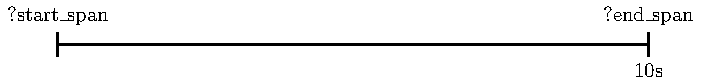
\includegraphics{tikz/start_end.pdf}
        \end{center}
        \caption{Execution of a long span in OpenTelemetry, the user will only be notified after 10 seconds that the function has ended (and taken too long).}
    \end{figure}

    \begin{figure}[H]
        \begin{center}
            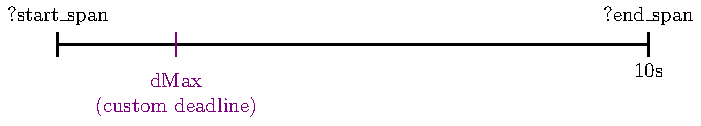
\includegraphics{tikz/start_end_dmax.pdf}
        \end{center}
        \caption{Execution of a long span in OpenTelemetry, the $dMax$ deadline allows knowing that the span has taken too long.}
        \label{fig:otel_dmax}
    \end{figure} 


    \subsection{Handling of long span}
        OpenTelemetry presents a bigger problem, what happens when there are long-running spans? Worse, what happens when spans are not actually terminated?
        
        OpenTelemetry limits the length of its spans, moreover, those who are not terminated are lost and not exported. Why? All spans must be ended!

        If the span is the parent/root span, its effect could trickle down to child spans. We can quickly see how this becomes problematic, all the information about an execution of your program \dots lost. Moreover, a span could not be terminated for trivial reasons: refreshing a tab, network failures, crashes \dots \cite{otel-l}. There are a few hacks that can be implemented, having shorter spans, carrying data in child spans, saving spans in a log to track spans which were not ended to manually set an end time; why the need to circumvent limitations when observing a system?

        These problems are a big limitation of OpenTelemetry, we believe that the wrapper we provide can be a great start to improve observability requirements in OpenTelemetry.
